

\chapter{Probability Theory}

	\section{Why Randomness and Probability?}
		\textbf{Probability Theory:}
		Mathematical framework for systems which behave in unpredictable or random ways
		
		\begin{itemize}
			\item \textbf{Most Sciences:} Systems too complex for exact modeling, lack of precise measurements
			\item \textbf{Computer Science:} Randomness is a resource
			\item \textbf{Cryptography:} Impossible without randomness!
		\end{itemize}
	
	\section{How can randomization lead to efficient algorithms?}
		\begin{itemize}
			\item Example: Election Winners
			\item You have an election with 40 million voters and want to know quickly who is the (likely) winner
			\item You want to know who the winner is without counting all votes
			\item Idea: Take a \textbf{random sample} of 1000 votes determine the winner!
		\end{itemize}
	
	\section{Probability Spaces}
		A finite probability space consists of two components:
		\begin{enumerate}
			\item A finite set $\Omega$ called the sample space.
			\item A probability function $Pr: \Omega \to \mathbb{R}$ satisfying
				\begin{itemize}
					\item For all $\omega \in \Omega$: $0 \leq Pr[\omega] \leq 1$
					\item $\sum\limits_{\omega \in \Omega} Pr[\omega] = 1$
				\end{itemize}
		\end{enumerate}
		\begin{itemize}
			\item The $\omega\in \Omega$ are called elementary events or outcomes
			\item A set $E \subseteq \Omega$ is called event
			\item For an event $E$ define
				\begin{center}
					$Pr[E] = \sum\limits_{\omega \in E} Pr[\omega]$
				\end{center}
				where $Pr[\emptyset] = 0$
		\end{itemize}
	
	\section{Set Operations on events}
		\begin{itemize}
			\item The intersection $E_1 \cap E_2$ of two events $E_1$ and $E_2$ is interpreted as the logical "and" of two events.
			Depending on the context, we will use the following notations
			\begin{center}
				$Pr[E_1 \cap E_2] =: Pr[E_1,E_2] =: Pr[E_1 \wedge E_2] =: Pr[E_1 \  and \  E_2]$
			\end{center}
			\item The union $E_1 \cup E_2$ of two events $E_1$ and $E_2$ is interpreted as the logical "or" of two events.
			Thus, we will use the following notation
			\begin{center}
				$Pr[E_1 \cup E_2] =: Pr[E_1 \vee E_2] =: Pr[E_1 \  or \  E_2]$
			\end{center}
			\item The complement $\bar{E} = \Omega \backslash E$ of an event $E$ is interpreted as the logical "negation" of $E$.
			We will use the notation
			\begin{center}
				$Pr[\bar{E}] =: Pr[\neg E] =: Pr[not \  E]$
			\end{center}
			\item If $A \subseteq B$ we say that the event $A$ implies the event $B$ and also write $A \Rightarrow B$
		\end{itemize}
	
	\section{Properties of Probability Spaces}
		\begin{itemize}
			\item For all events $A,B \subseteq \Omega$:
				\begin{enumerate}
					\item $Pr[A \cup B] = Pr[A] + Pr[B] - Pr[A \cap B]$
					\item $Pr[\bar{A}] = 1 - Pr[A]$
					\item If $A \subseteq B$ then $Pr[A] \leq Pr[B]$
				\end{enumerate}
			\item Item 1 implies the \textbf{union-bound}:\\
			For all $A,B \subseteq \Omega$ it holds $Pr[A \cup B] \leq Pr[A] + Pr[B]$
		\end{itemize}
	
	\section{Conditional Probabilities and Independence}
		\begin{itemize}
			\item For two events $A$ and $B$ we define the conditional probability 
			\begin{center}
				$Pr[A|B] = \frac{Pr[A \cap B]}{Pr[B]}$, $Pr[B] > 0$
			\end{center}
			\item Two events $A,B \subseteq \Omega$ are called independent if
			\begin{center}
				$Pr[A \cap B] = Pr[A] \cdot Pr[B]$
			\end{center}
			\item This is equivalent to $Pr[A|B] = Pr[A]$
			\item By symmetry also to $Pr[B|A] = Pr[B]$
		\end{itemize}

	\section{Bayes' Rule}
		\begin{itemize}
			\item Bayes’ rule relates the conditional probabilities $Pr[A|B]$ and $Pr[B|A]$
			\item This is especially useful when analyzing larger processes composed of smaller ones
		\end{itemize}
		\textbf{Bayes' Rule}\newline
		For all $A,B \subseteq \Omega$, it holds for $Pr[A],Pr[B] > 0$, that
		\begin{center}
			$Pr[A|B] = \frac{Pr[B|A] \cdot Pr[A]}{Pr[B]}$
		\end{center}
		
		\begin{proof}
		$Pr[A|B] = \frac{Pr[A \cap B]}{Pr[B]} \cdot \frac{Pr[A]}{Pr[A]} = \frac{Pr[A \cap B]}{Pr[A]} \cdot \frac{Pr[A]}{Pr[B]} 
		= \frac{Pr[B \cap A]}{Pr[A]} \cdot \frac{Pr[A]}{Pr[B]} = \frac{Pr[B|A] \cdot Pr[A]}{Pr[B]}$
		\end{proof}
		
	\section{Law of Total Probability}
		\begin{itemize}
			\item Sometimes we want to infer the probability of an event given conditional probabilities of this event
			\item This will also be useful to compute/bound probabilities by a case analysis
		\end{itemize}
		\textbf{Law of Total Probability}\newline
		Let $B_1,...,B_n$ be events that partition the probability space $\Omega$, i.e. $B_1 \cup ... \cup B_n = \Omega$ and $B_i \cap B_j = \emptyset$ for $i \neq j$.
		Then it holds for every event $A$ that
		\begin{center}
			$\sum\limits_{i=1}^{n} Pr[A \cap B_i] = Pr[A]$, with $Pr[A \cap B_i] = Pr[A|B_i] \cdot Pr[B_i]$
		\end{center}
		
		\begin{proof}\ Preconditions:
			\begin{enumerate}
				\item $Pr[E_1 \cup E_2] Pr[E_1] + Pr[E_2]$ if $E_1 \cap E_2 = \emptyset$, and
				\item $Pr[E_1 \cup ... \cup E_n] = \sum\limits_{i=1}^{n} Pr[E_i]$ if $E_i \cap E_j = \emptyset$ for $i \neq j$.
				\item $Pr[A \cap B_i] = Pr[A|B_i] \cdot Pr[B_i]$
			\end{enumerate}
			We know that $A = A \cap \Omega = A \cap \Big( \bigcup\limits_{i=1}^{n} B_i \Big) = \bigcup\limits_{i=1}^{n} A \cap B_i$.\\
			So it follows $Pr[A] = Pr\Big[\bigcup\limits_{i=1}^{n} A \cap B_i\Big] \overset{\text{(2.)}}{=} \sum\limits_{i=1}^{n} Pr[A \cap B_i] 
			\overset{\text{(3.)}}{=} \sum\limits_{i=1}^{n} Pr[A | B_i]\cdot Pr[B_i]$.
		\end{proof}
		
	\section{Example: Bayes and LotP in Action}
		\begin{itemize}
			\item Assume 2 in 1000 people in a population have a certain disease
			\item There exists a test for this disease but it is not flawless
			\item If you have the disease, then there is a 95$\%$ chance that the test returns positive
			\item Moreover, there is a 3$\%$ chance that the test returns positive even if you don t have the disease
			\item Imagine, you do a test and it returns positive, what is the probability that you actually have the disease?
		\end{itemize}
		\textbf{Remarks:}
		\begin{itemize}
			\item The probability 2 1000 = 0.002 is your prior of having the disease, i.e. if you do not get the additional information of test, this is your best guess
			\item We are interested in the posterior probability
		\end{itemize}
		\textbf{Solution:}
		\begin{itemize}
			\item Let s model this with a probability space
			\item Let $A$ be the event that you have the disease. We know that $Pr[A] = 0.002$
			\item Let $B$ be the event that the test returns positive. We know that $Pr[B|A] = 0.95$
			\item We also know that $Pr[B|\bar{A}] = 0.03$
			\item We want to know the posterior $Pr[A|B]$
		\end{itemize}
		$Pr[A|B] = \frac{Pr[B|A] \cdot Pr[A]}{Pr[B]} = \frac{Pr[B|A] \cdot Pr[A]}{Pr[B|A] \cdot Pr[A] + Pr[B|\bar{A}] \cdot Pr[\bar{A}]} 
		= \frac{Pr[B|A] \cdot Pr[A]}{Pr[B|A] \cdot Pr[A] + Pr[B|\bar{A}] \cdot (1-Pr[A])} \approx 0.06$\\
		
		If you do a test and it returns positive, the probability that you actually have the disease is $6\%$!
		
	\section{Summary 1}
		\begin{itemize}
			\item Probability spaces model randomized processes
			\item Conditional probabilities tell us a posteriori probabilities given that some event has happened
			\item Bayes’ rule and the law of total probability simplify working with conditional probabilities
		\end{itemize}

\newpage

	\section{Random Variables}
		\begin{itemize}
			\item In general, any function $X: \Omega \to D$ for some domain $D$ is called a ($D$-valued) \textbf{random variable}
			\item We can now define events with respect to a random variable.
			\item Let $x \in D$ define the event $E_x = \{ \omega \in \Omega: X(\omega)=x \} \subseteq \Omega$
			\item We write the shorthand $X=x$ for $E_x$
			\item We call the function $F(x) = Pr[E_x] = Pr[X=x]$ the probability distribution of $X$
		\end{itemize}
	
		\subsection{Independence of random variables}
			\begin{itemize}
				\item Consider two random variables $X \in D_X$ and $Y \in D_Y$, which means $X: \Omega \to D_X$ and $Y: \Omega \to D_Y$
				\item We say that $X$ and $Y$ are \textbf{independent}, if it holds for all $x \in D_X$ and $y \in D_Y$ that the events $X=x$ and $Y=y$ are independent
				\item I.e. $Pr[X=x,Y=y] = Pr[X=x] \cdot Pr[Y=y]$
			\end{itemize}
		
		\subsection{Examples}
			\begin{itemize}
				\item \textbf{Identity function:}\\
					$X: \Omega \to \Omega$. In this case $Pr[X=\omega] = Pr[\omega]$.
				\item \textbf{Projections:}\\
					Let $\Omega \subseteq D_1 \times D_2$, then $X: \Omega \to D_1$, $(x,y) \mapsto x$ and $Y: \Omega \to D_2$, $(x,y) \mapsto y$ are projections.
				\item \textbf{Reverse direction:}\\
					Given two sample spaces $\Omega_1$ and $\Omega_2$, we can form a new sample space $\Omega = \Omega_1 \times \Omega_2$.\\
					Then the projections $X: \Omega \to \Omega_1$ and $Y: \Omega \to \Omega_2$ are independent random variables.
				\item We say that a random variable $X: \Omega \to D$ is \textbf{uniform} on $D$ or an \textbf{uniform distribution}, if for every $x \in D$ 
					it holds $Pr[X=x] = \frac{1}{|D|}$
				\item \textbf{Sum of two dice rolls:}\\
					Let $\Omega = \{1,...,6\} \times \{1,...,6\}$, then $S: \Omega \to \mathbb{Z}$ with $(x,y) \mapsto x+y$ is a sum of two dice rolls.
				\item \textbf{Indicator random variable:}\\
				For an event $E$ we can define the random $X_E: \Omega \to \{0,1\}$ such that $X_E(\omega)=1$ if $\omega \in E$ and $X_E(\omega)=0$ if $\omega\notin E$
			\end{itemize}
		
		\subsection{Defining Probability Spaces via Random Variables}
			\begin{itemize}
				\item From now on we will omit the function notation for random variables
				\item Moreover, from now on we will also omit defining the sample space $\Omega$ explicitly
				\item Instead, we implicitly define $\Omega$ via a set of random variables
				\item General idea: The probability space is defined via a few independent "base" random variables
				\item All other random variables of interest depend on these deterministically
				\item When constructing a system that uses randomization, we do not need to keep track of the sample space, it is define "on the fly" as we introduce new random
				variables
				\item If $X$ is chosen uniformly random from some domain $D$, we will use the notation $X \leftarrow_{\$} D$ instead of the function notation
			\end{itemize}
		
		\subsection{Examples}
			\begin{itemize}
				\item Let $X_1,...,X_n$ be independent random variables such that each $X_i$ is uniform on $\{ 0,1 \}$.
				We say $X_1,...,X_n$ are \textbf{iid uniform on} $\{0,1\}$ for short
				\item Then $X = (X_1,...,X_n)$ is uniform on $\{0,1\}^n$
				\item $Y = X_1 + ... + X_n$ follow a distribution which is called the Bernoulli distribution
			\end{itemize}
			\begin{center}
				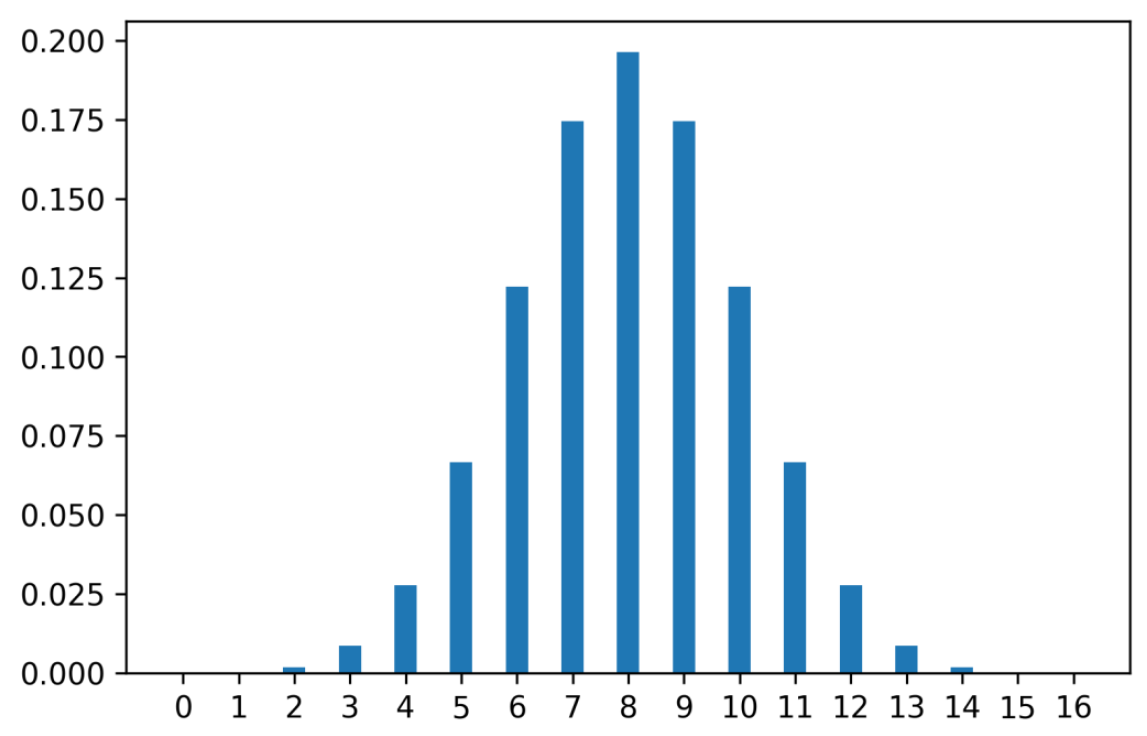
\includegraphics[width=120mm]{Graphics/Probability Theory/Examples1.png}\newline
			\end{center}
		
		\subsection{Sampling Algorithms}
			\begin{itemize}
				\item In general: We say a random variable $Z$ is \textbf{sampleable}, if there exists an (efficient) algorithm $M$ such that
				$Z = M(X_1,...,X_n)$, where $X_1,...,X_n$ are iid uniform on $\{0,1\}$
				\item $X_1,...,X_n$ are called the \textbf{random coins} or just \textbf{coins} of $M$
			\end{itemize}
			\begin{center}
            	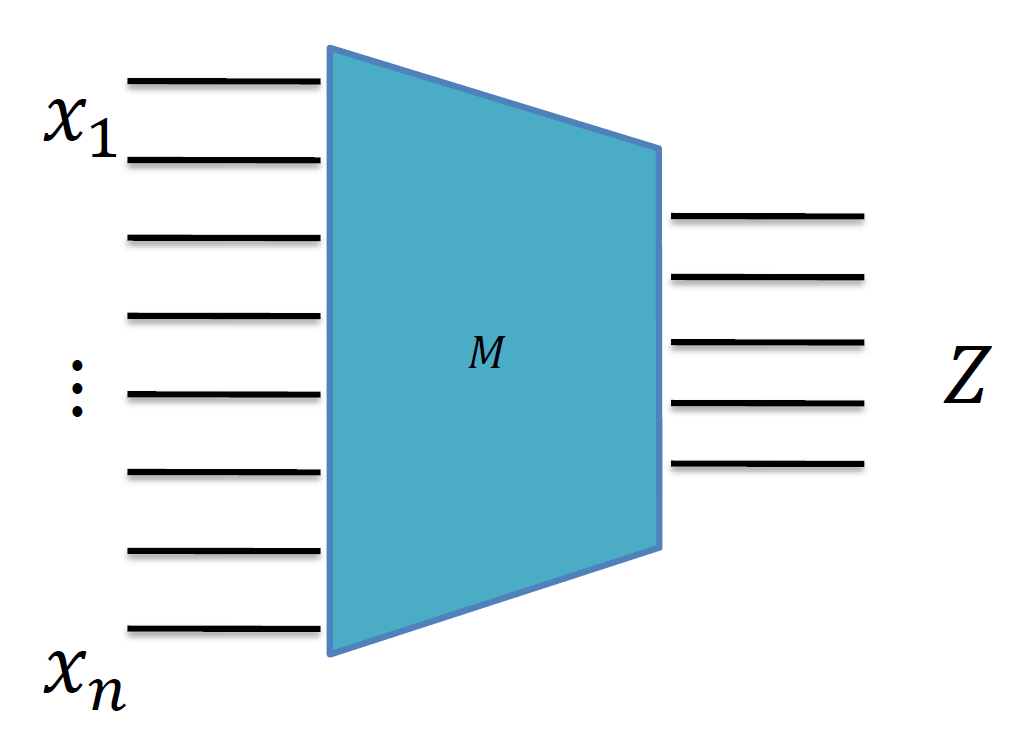
\includegraphics[width=120mm]{Graphics/Probability Theory/SamplingAlgorithms.png}\newline
        	\end{center}
        
	\section{Real-Valued Random Variables and Expectations}
		\begin{itemize}
			\item We call random variables $X: \Omega \to \mathbb{R}$ \textbf{real-valued}
			\item We call $Supp(X) = X(\Omega) \subseteq \mathbb{R}$ the \textbf{support} of $X$
			\item Note that $Supp(X)$ is finite as $\Omega$ is finite
			\item For a real-valued random variable $X$, we can define an \textbf{expectation}
				\begin{center}
					$E[X] = \sum\limits_{x \in Supp(X)} x \cdot Pr[X=x]$
				\end{center}
		\end{itemize}
		
		\subsection{Linearity of Expectation}
			\begin{itemize}
				\item Expectations are characteristic of random variables
				\item Powerful tool to analyze random variables constructed from other random variables
			\end{itemize}
			\textbf{Linearity of Expectation}\\
			Let $X$ and $Y$ be two real-valued random variables and $\alpha \in \mathbb{R}$ be a constant.\\
			Then it holds that
			\begin{enumerate}
				\item $E[\alpha \cdot X] = \alpha \cdot E[X]$
				\item $E[X+Y] = E[X]+E[Y]$
			\end{enumerate}
			Note: $X$ and $Y$ don't need to be independent
			
			\begin{proof}
			Proof of the linearity properties of expectation
			\begin{enumerate}
				\item To show: $E[\alpha \cdot X] = \alpha \cdot E[X]$
					\begin{align*}
						E[\alpha \cdot X] &= \sum\limits_{z \in Supp(\alpha \cdot X)} z \cdot Pr[\alpha \cdot X = z] \text{, with } \alpha \neq 0
					\end{align*}
					Now we make the following substitution: $z = \alpha \cdot z'$
					\begin{align*}
						E[\alpha \cdot X] &= \sum\limits_{z'} \alpha \cdot z' \cdot Pr[\alpha \cdot X = \alpha \cdot z']\\
						&= \alpha \cdot \sum\limits_{z'} \cdot Pr[X=z']\\
						&= \alpha \cdot E[X]
					\end{align*}
				
				\item To show: $E[X+Y] = E[X]+E[Y]$
					\begin{align*}
						E[X] &= \sum\limits_{x \in Supp(x)} x \cdot Pr[X=x]\\
						&= \sum\limits_{x \in S} x \cdot Pr[X=x] \text{, with } Supp(X),Supp(Y),Supp(X+Y) \leq S
					\end{align*}
					\begin{align*}			
						E[X+Y] &= \sum\limits_{z \in Supp(X+Y)} z \cdot Pr[X+Y = z]\\
						&= \sum\limits_{y \in Supp(Y)} \sum\limits_{z \in Supp(X+Y)} z \cdot Pr[X=z-y \wedge Y=y]\\
						&= \sum\limits_{y \in S} \sum\limits_{x \in S} (x+y) \cdot Pr[X=x, Y=y] \text{, with } z=x+y\\
						&= \sum\limits_{y \in S} \sum\limits_{x \in S} x \cdot Pr[X=x, Y=y] + \sum\limits_{y \in S} \sum\limits_{x \in S} y \cdot Pr[X=x, Y=y]\\
						&= \sum\limits_{x \in S} x \cdot \sum\limits_{y \in S} Pr[X=x, Y=y] + \sum\limits_{y \in S} y \cdot \sum\limits_{x \in S} Pr[X=x, Y=y]\\
						&= \sum\limits_{x \in S} x \cdot Pr[X=x] + \sum\limits_{y \in S} y \cdot Pr[Y=y]\\
						&= E[X] + E[Y]
					\end{align*}
			\end{enumerate}
			\end{proof}
		
		\subsection{Example}
			\begin{itemize}
				\item Let $X_1,...,X_n$ be independently distributed random variables on $\{0,1\}$ such that for all $i$ it holds $Pr[X_i=1] = p$ for a constant $p \in [0,1]$
				\item What is the expectation of $Y = X_1+...+X_n$?\\
					$E[Y] = E[X_1+...+X_n] = E[X_1] +...+ E[X_n] = n \cdot p$\\
					$Pr[X_i = 1] = p \Rightarrow E[X_i] = \sum\limits_{b \in \{0,1\}} b \cdot Pr[X_i = b] = Pr[X_i = 1] = p$
			\end{itemize}

	\section{A little detour to Algebra: Finite Groups}
		\subsection{Groups}
			A set $G$ together with a binary operation $\circ: G \times G \to G$ is called a group, if the following conditions are met:
			\begin{enumerate}
				\item \textbf{Associativity:} 
				For all $f,g,h \in G$ it holds that $(f \circ g) \circ h = f \circ (g \circ h)$
				\item \textbf{Identity Element:} 
				There exists a special element $e \in G$ such that for all $g \in G$ it holds $e \circ g = g \circ e = g$
				\item \textbf{Inverses Element:}
				For every $g \in G$ there exists an element $g^{-1} \in G$ such that $g \circ g^{-1} = e$
			\end{enumerate}
			\begin{itemize}
				\item A group $(G,\circ)$ is called \textbf{commutative (abelian) group} if for all $g,h \in G$ it holds $g \circ h = h \circ g$
				\item We say a group $(G,\circ)$ is \textbf{finite} if $G$ is finite as a set
			\end{itemize}
		
		\subsection{Examples of Groups}
			\begin{itemize}
				\item The integers under addition: $(\mathbb{Z},+)$
				\item Modular integers under addition: $(\mathbb{Z}/n\mathbb{Z}, +\ mod\ n)$
				\item The non-zero rational numbers under multiplication: $(\mathbb{Q} \backslash \{0\}, \cdot)$
				\item The binary set under XOR: $(\{0,1\}, \oplus)$
				\item Binary vectors under XOR: $(\{0,1\}^n, \oplus)$ with $\oplus$ bitwise
			\end{itemize}
		
		\subsection{Random Variables in Groups}
			\begin{itemize}
				\item Let $U$ be uniformly distributed on a \textbf{finite group} $G$
				\item I.e. for all $g \in G$ it holds $Pr[U=g] = \frac{1}{|G|}$
				\item Fix an $z \in G$, what is the probability distribution of $U \circ z$?
				\item $\Rightarrow$ If $U$ is uniformly distributed on $G$ and $Z$ is a random variable supported on $G$ and independent of $U$, 
				then $U \circ Z$ is also uniformly distributed on $G$
				\item In particular for $G = \{0,1\}$ and $\circ = \oplus$, $U \oplus Z$ is distributed uniformly random.
			\end{itemize}
	
	\section{Summary 2}
		\begin{itemize}
			\item Random variables are "the right way" to define and work with probability spaces
			\item In CS, we usually define all variables depending on some uniform and independent "base variables"
			\item For real valued random variables we can compute expectations
			\item Expectations are linear
			\item XOR-ing a uniformly random and independent variable onto something else results again in a uniform distribution.
		\end{itemize}
















































